\documentclass[aspectratio=169, 9pt]{beamer}

% Пакеты для русского языка
\usepackage[T2A]{fontenc}
\usepackage[utf8]{inputenc}
\usepackage[russian]{babel}

% Светлая тема
\usetheme{Ilmenau}
\usecolortheme{default}

% Цвета
\setbeamercolor{background canvas}{bg=white}
\setbeamercolor{normal text}{fg=black}
\setbeamercolor{frametitle}{fg=blue!80!black, bg=blue!5}
\setbeamercolor{title}{fg=white!80!black}
\setbeamercolor{item}{fg=blue!70}
\setbeamercolor{subitem}{fg=green!50!black}

% Шрифты
\usefonttheme{professionalfonts}
\setbeamerfont{title}{size=\large, series=\bfseries}
\setbeamerfont{frametitle}{size=\normalsize, series=\bfseries}

% Убираем навигацию
\setbeamertemplate{navigation symbols}{}

% Футер
\setbeamertemplate{footline}{
  \leavevmode%
  \hbox{%
    \begin{beamercolorbox}[wd=.33\paperwidth,ht=2ex,dp=1ex,center]{author in head/foot}%
      \insertshortauthor
    \end{beamercolorbox}%
    \begin{beamercolorbox}[wd=.34\paperwidth,ht=2ex,dp=1ex,center]{title in head/foot}%
      \insertshorttitle
    \end{beamercolorbox}%
    \begin{beamercolorbox}[wd=.33\paperwidth,ht=2ex,dp=1ex,right]{date in head/foot}%
      \insertframenumber{} / \inserttotalframenumber\hspace*{2ex}
    \end{beamercolorbox}}%
  \vskip0pt%
}

% Пакеты
\usepackage{graphicx}
\usepackage{amsmath}

\title{Основные задачи Computer Vision}
\subtitle{Нейронные сети в компьютерном зрении}
% \author{Презентация для студентов}
\date{2026}

\begin{document}

% Слайд 1: Титульный
\begin{frame}
\titlepage
\end{frame}

% Слайд 2: Введение
\begin{frame}{Введение в Computer Vision}
\begin{columns}[T]
\begin{column}{0.5\textwidth}
{\bfseries\textcolor{blue!70}{Что такое Computer Vision?}}

{\small Преобразование визуальных данных в высокоуровневое понимание сцены.}

\vspace{0.5em}
{\bfseries\textcolor{blue!70}{Как работают нейросети}}

{\small
\begin{itemize}
    \item Автоизвлечение признаков
    \item Иерархия: Края $\to$ Текстуры $\to$ Объекты
    \item Обучение на размеченных данных
\end{itemize}
}
\end{column}

\begin{column}{0.5\textwidth}
{\bfseries\textcolor{green!50!black}{Почему эффективны нейросети}}

{\small
\begin{itemize}
    \item Устойчивость к вариациям
    \item Обобщающая способность
    \item Масштабируемость
\end{itemize}
}

\vspace{0.5em}
{\bfseries\textcolor{blue!70}{Типы задач}}

{\small
\begin{itemize}
    \item Classification (Классификация)
    \item Detection (Детекция)
    \item Segmentation (Сегментация)
\end{itemize}
}
\end{column}
\end{columns}
\end{frame}

% Слайд 3: Основные задачи
\begin{frame}{Основные задачи Computer Vision}
\begin{columns}[T]
\begin{column}{0.45\textwidth}
{\bfseries\textcolor{blue!70}{1. Классификация}}

{\small Сеть выдает вероятности для каждого класса через softmax}

{\small\textit{Пример:} «Кошка» = 0.95, «Собака» = 0.03}

\vspace{0.4em}
{\bfseries\textcolor{green!50!black}{2. Детекция объектов}}

{\small Локализация + Классификация}

{\small Предсказывает: Bounding box (x, y, w, h) + класс}
\end{column}

\begin{column}{0.55\textwidth}
{\bfseries\textcolor{blue!70}{3. Сегментация}}

{\small Попиксельная классификация}

{\small
\begin{itemize}
    \item \textbf{Семантическая:} Все объекты одного класса одного цвета
    \item \textbf{Instance:} Каждый объект уникальный цвет
\end{itemize}
}

\vspace{0.3em}
\centering
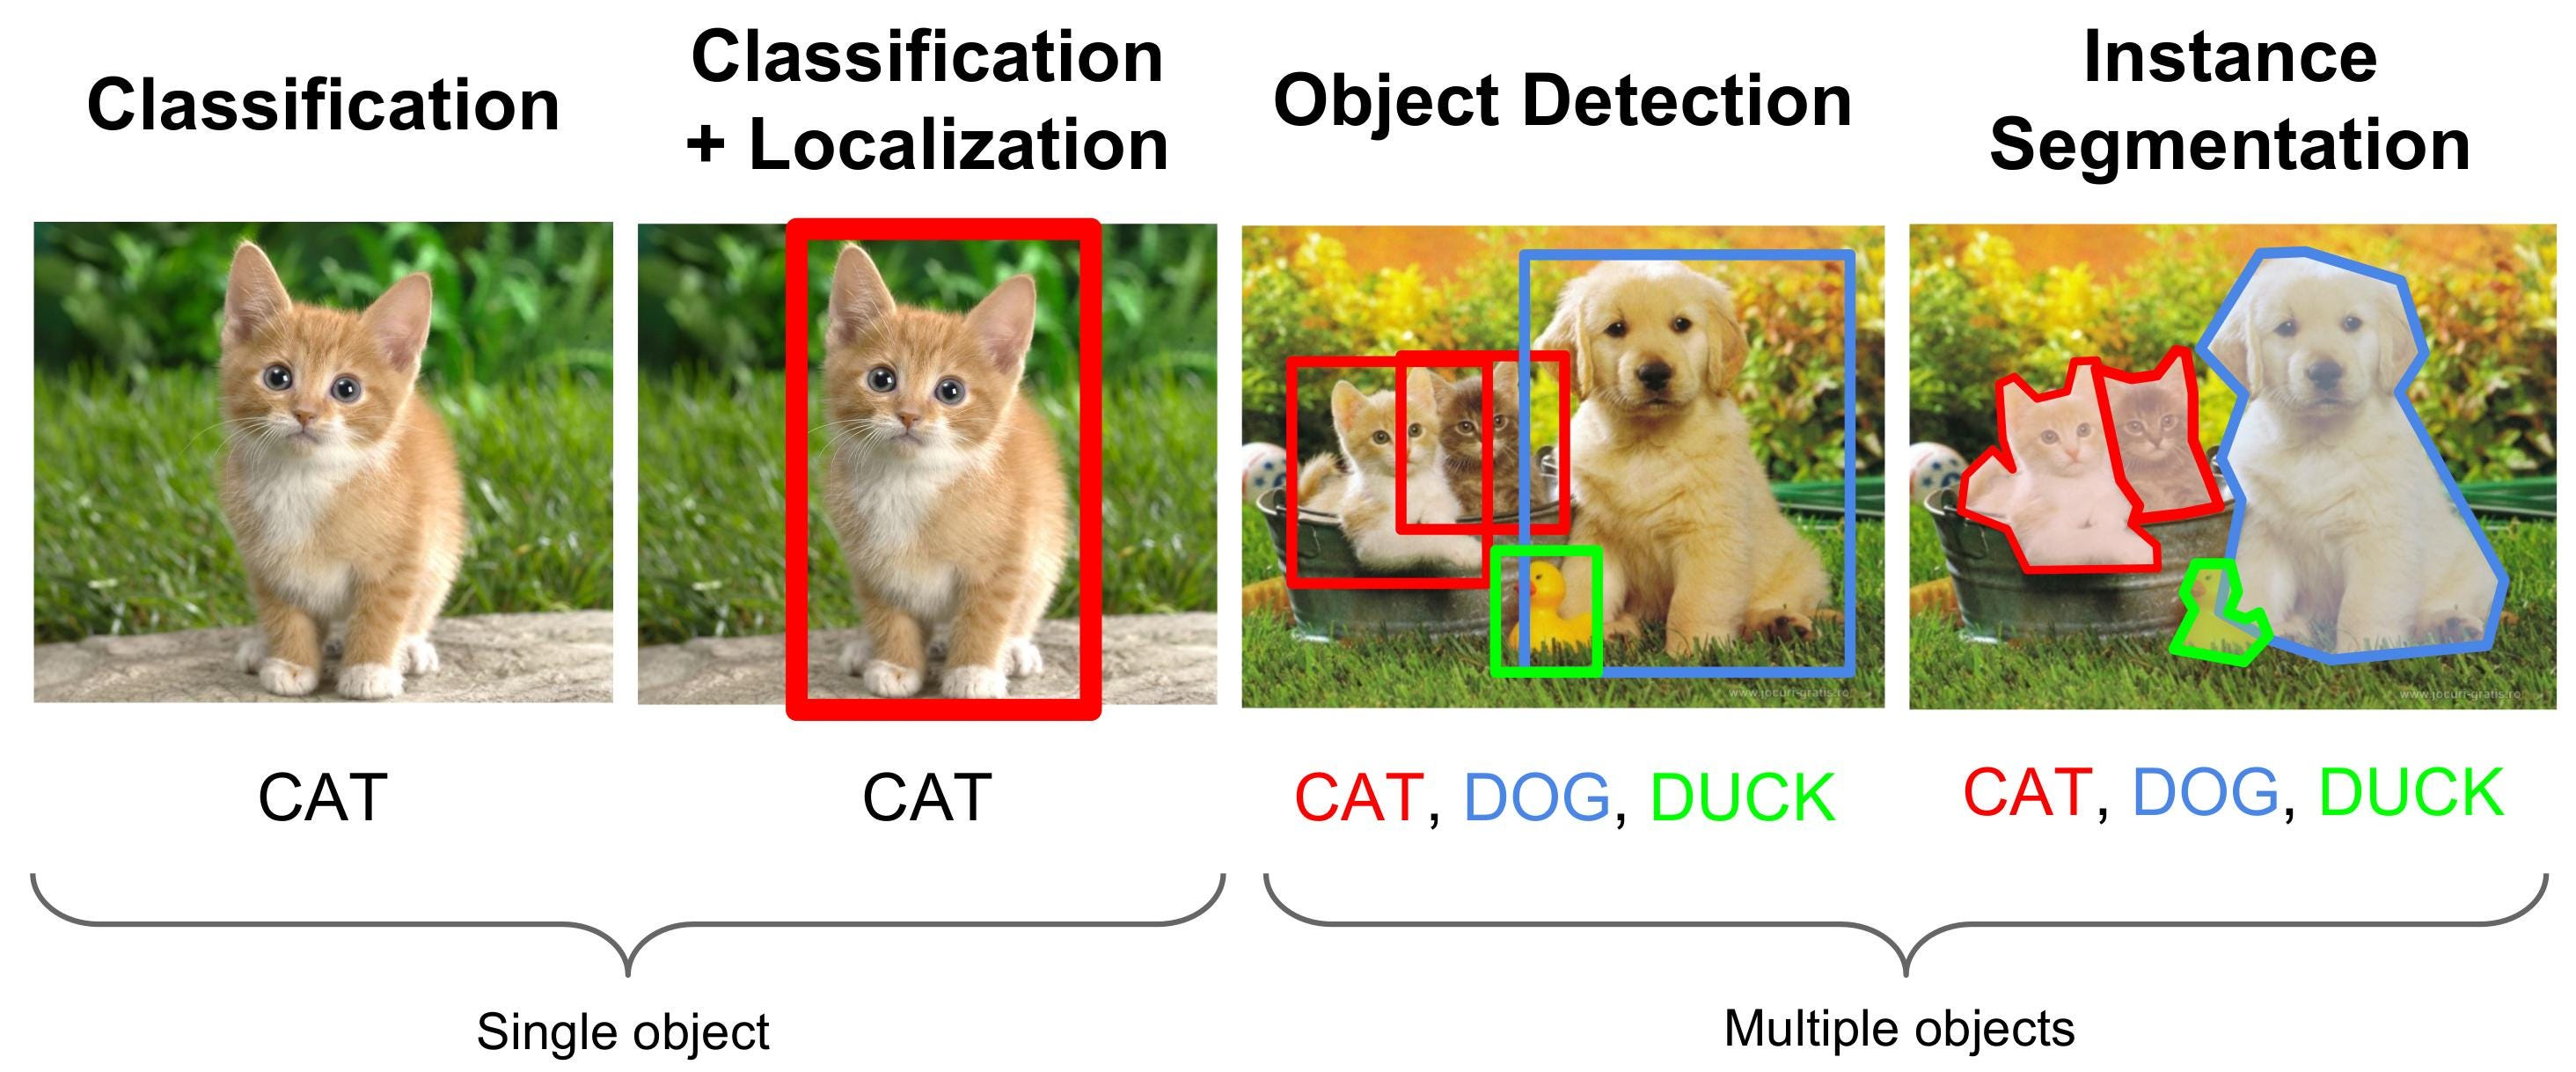
\includegraphics[width=0.7\textwidth]{images/cv_tasks_comparison.jpeg}
\end{column}
\end{columns}
\end{frame}

% Слайд 4: Задачи (продолжение)
\begin{frame}{Основные задачи (продолжение)}
\begin{columns}[T]
\begin{column}{0.5\textwidth}
{\bfseries\textcolor{blue!70}{4. Распознавание лиц}}

{\small Embeddings $\to$ Distance comparison}

\vspace{0.3em}
{\bfseries\textcolor{green!50!black}{5. Детекция краев}}

{\small Gradient filters или CNN}

\vspace{0.3em}
{\bfseries\textcolor{blue!70}{6. Восстановление изображений}}

{\small Encoder-Decoder архитектура}

\vspace{0.3em}
{\bfseries\textcolor{green!50!black}{7. Сопоставление признаков}}

{\small Keypoint extraction + Matching}
\end{column}

\begin{column}{0.5\textwidth}
{\bfseries\textcolor{blue!70}{8. Реконструкция сцены}}

{\small Structure from Motion или Depth estimation}

\vspace{0.3em}
{\bfseries\textcolor{green!50!black}{9. Анализ движения}}

{\small Object tracking + Optical flow}

\vspace{0.5em}
\centering
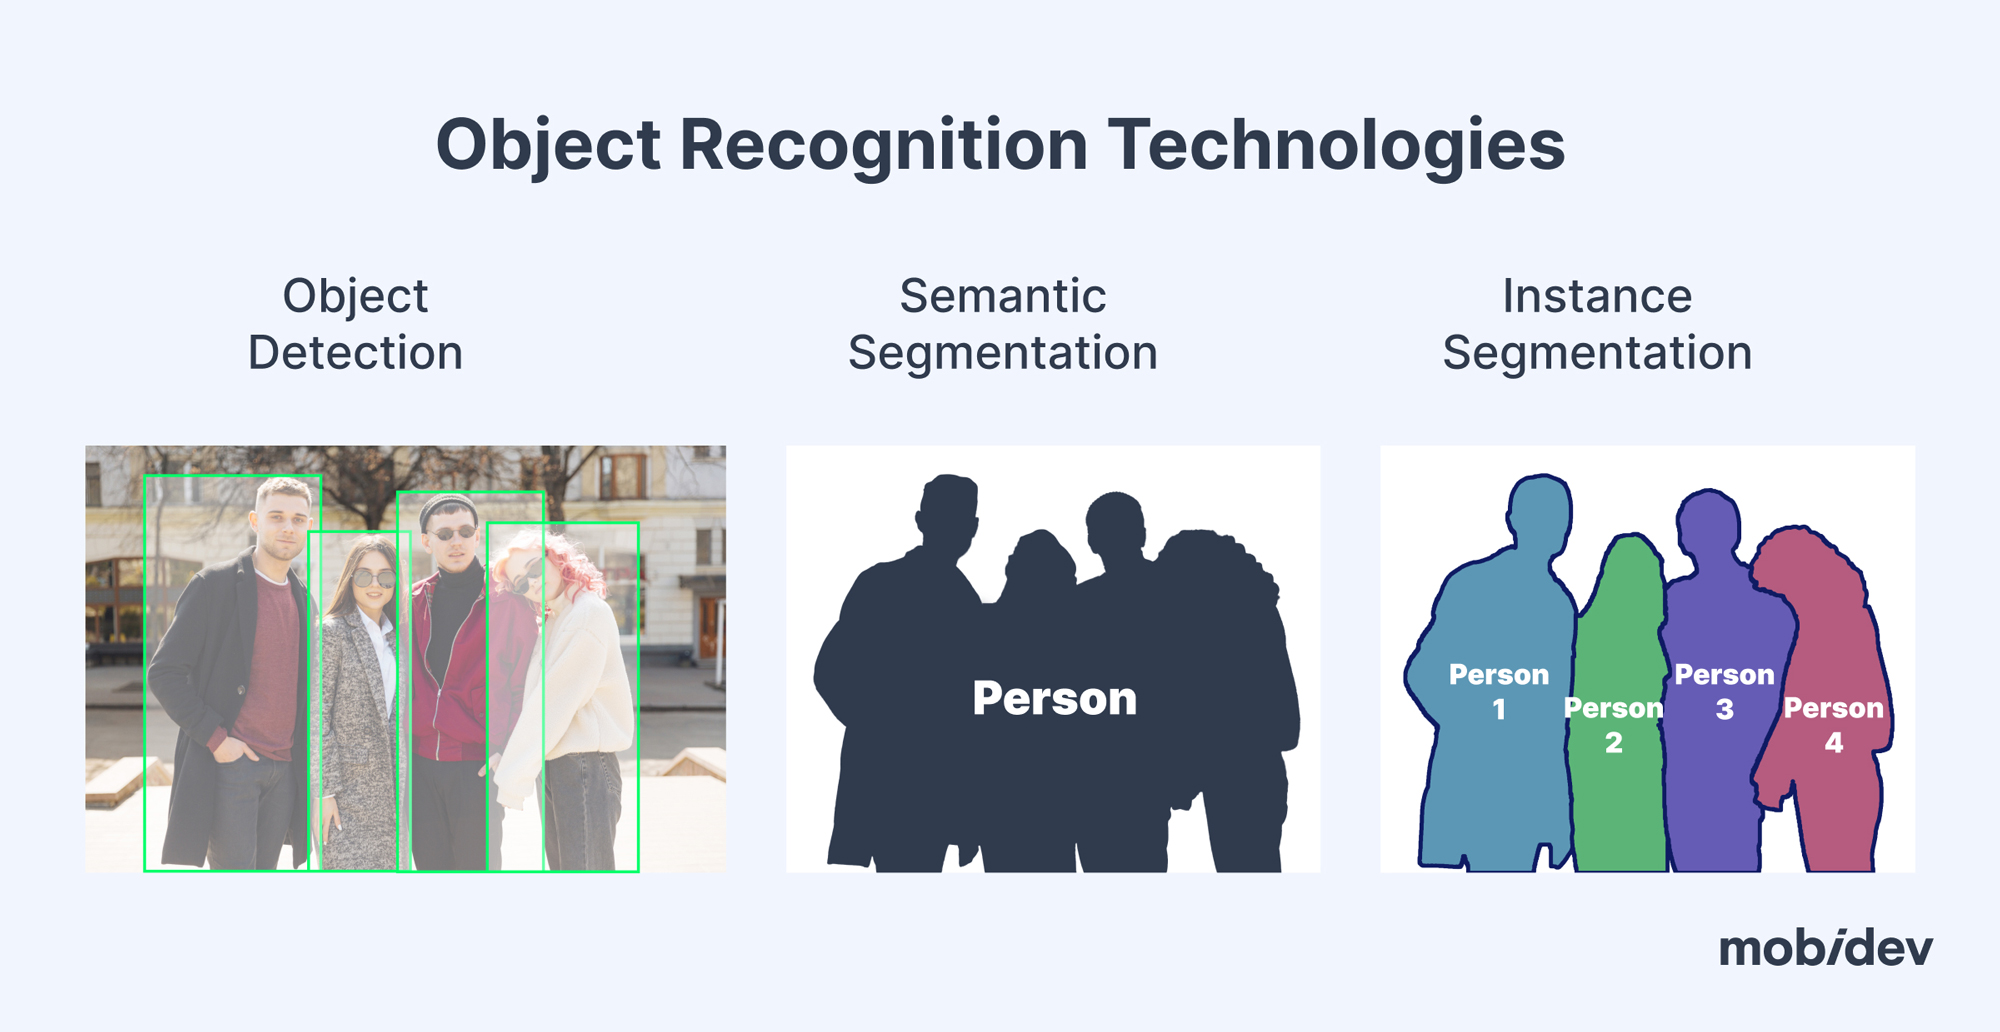
\includegraphics[width=0.65\textwidth]{images/cv_tasks_examples.png}
\end{column}
\end{columns}
\end{frame}

% Слайд 5: CNN
\begin{frame}{Сверточные нейронные сети (CNN)}
\begin{columns}[T]
\begin{column}{0.4\textwidth}
{\bfseries\textcolor{blue!70}{Иерархия признаков}}

{\small
\begin{itemize}
    \item Layer 1: Края, углы, цвета
    \item Layer 2-3: Текстуры, формы
    \item Layer 4-5: Части объектов
    \item FC: Целые объекты
\end{itemize}
}

\vspace{0.4em}
\centering
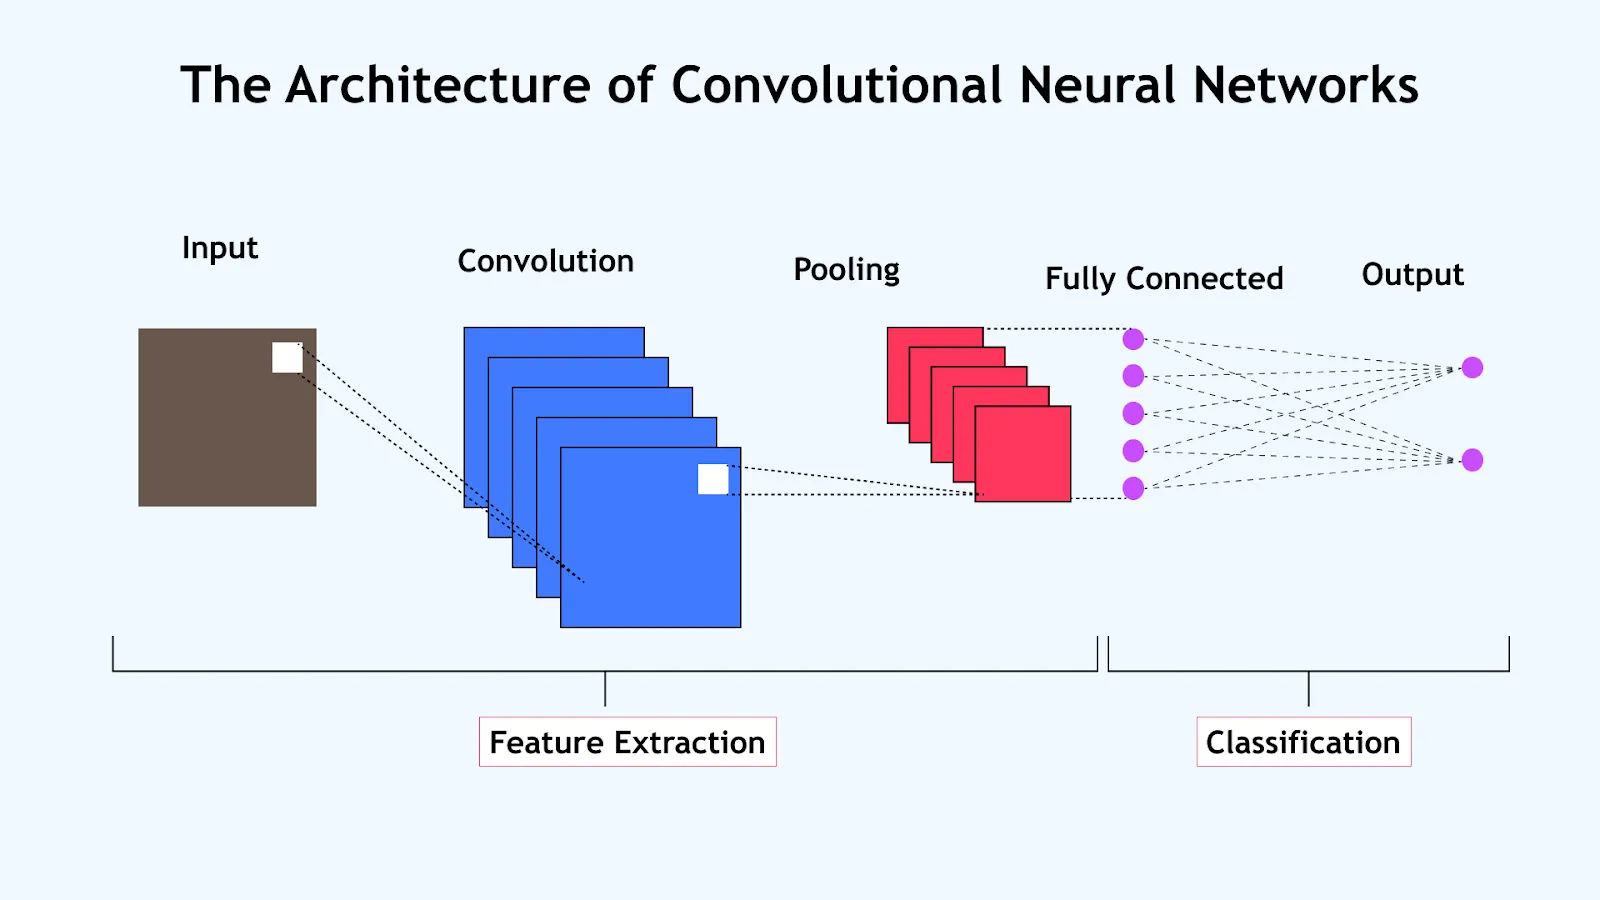
\includegraphics[width=0.75\textwidth]{images/cnn_architecture.png}
\end{column}

\begin{column}{0.6\textwidth}
{\bfseries\textcolor{blue!70}{Компоненты CNN}}

{\small
\begin{enumerate}
    \item \textbf{Сверточный слой:} Фильтры $\to$ Feature maps
    \item \textbf{ReLU:} $f(x) = \max(0, x)$     \item \textbf{Pooling:} Уменьшение размерности
    \item \textbf{FC слои:} Классификация
\end{enumerate}
}

\vspace{0.3em}
{\bfseries\textcolor{green!50!black}{Ключевые архитектуры}}

{\small
\begin{itemize}
    \item \textbf{ResNet:} Skip connections
    \item \textbf{Inception:} Параллельные свертки
    \item \textbf{EfficientNet:} Композитное масштабирование
\end{itemize}
}
\end{column}
\end{columns}
\end{frame}

% Слайд 6: Transfer Learning
\begin{frame}{Transfer Learning}
\begin{columns}[T]
\begin{column}{0.45\textwidth}
{\bfseries\textcolor{blue!70}{Идея}}

{\small Предобученная сеть уже умеет видеть края, текстуры, формы. Нужно адаптировать под задачу.}

\vspace{0.5em}
\centering
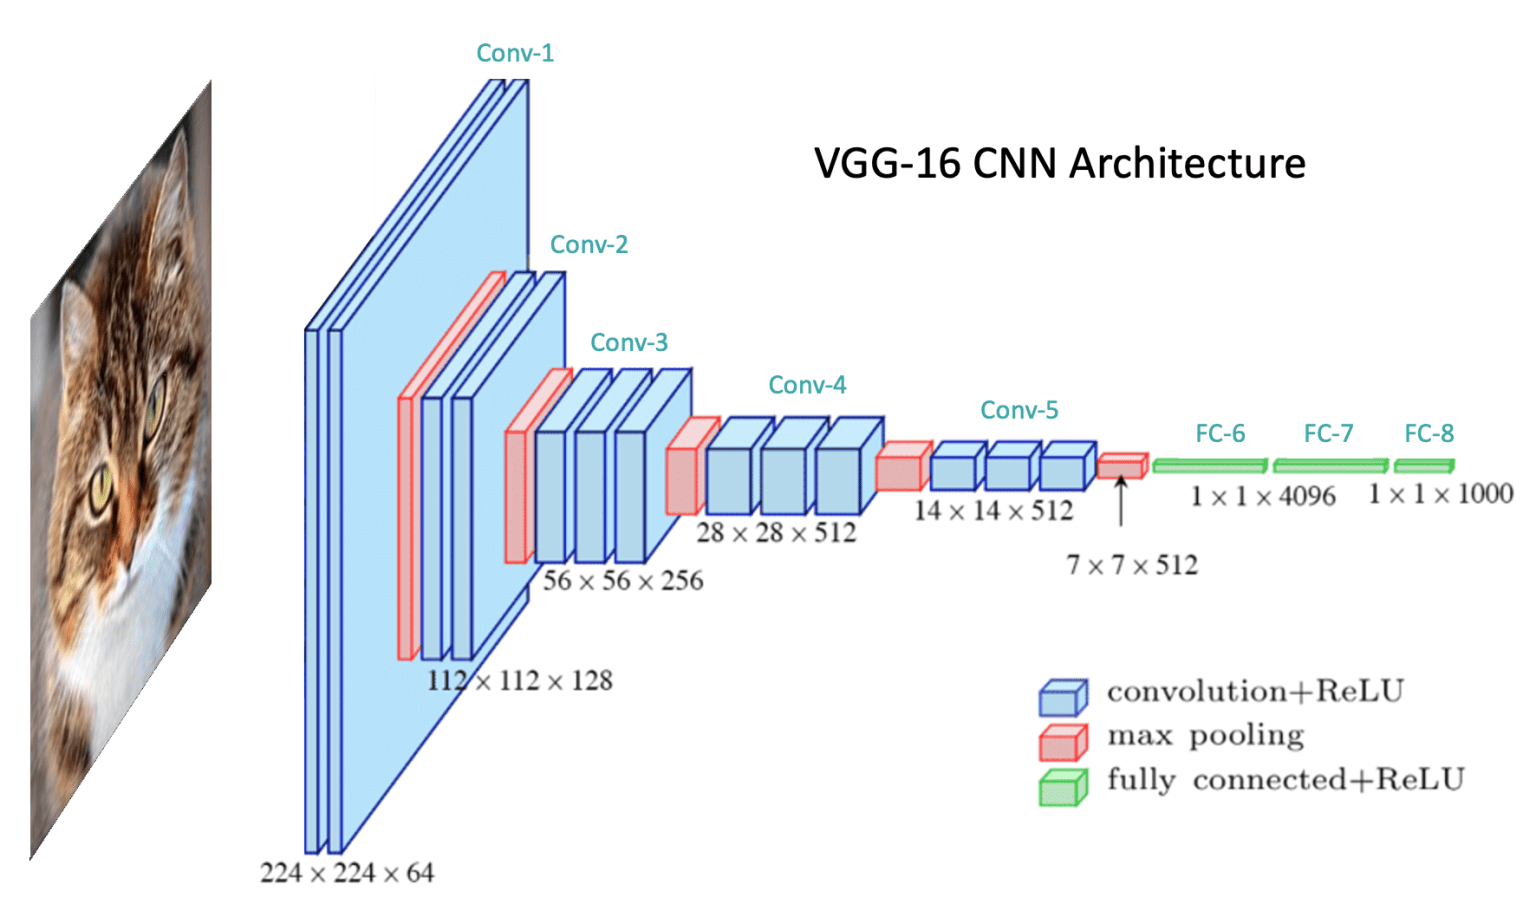
\includegraphics[width=0.7\textwidth]{images/vgg_architecture.png}
\end{column}

\begin{column}{0.55\textwidth}
{\bfseries\textcolor{blue!70}{1. Backbone}}

{\small Предобученная CNN: ResNet, VGG на ImageNet}

\vspace{0.3em}
{\bfseries\textcolor{green!50!black}{2. Стратегии обучения}}

{\small
\begin{itemize}
    \item \textbf{Freeze:} Фиксируем ранние слои
    \item \textbf{Fine-tune:} Обучаем поздние слои
\end{itemize}
}

\vspace{0.3em}
{\bfseries\textcolor{blue!70}{3. Замена головы}}

{\small
\begin{itemize}
    \item Classification: Новые FC слои
    \item Detection: RPN + classifier
    \item Segmentation: Decoder
\end{itemize}
}
\end{column}
\end{columns}
\end{frame}

% Слайд 7: Детекция объектов
\begin{frame}{Архитектуры для детекции объектов}
\begin{columns}[T]
\begin{column}{0.5\textwidth}
{\bfseries\textcolor{blue!70}{Двухстадийные}}

{\small\textbf{Faster R-CNN:}}
{\small
\begin{itemize}
    \item RPN генерирует anchor boxes
    \item ROI Pooling извлекает признаки
    \item Классификатор: класс + координаты
\end{itemize}
}

\vspace{0.3em}
{\small\textit{Процесс:} RPN $\to$ Regions $\to$ ROI $\to$ Output}
\end{column}

\begin{column}{0.5\textwidth}
{\bfseries\textcolor{green!50!black}{Одностадийные}}

{\small\textbf{YOLO:}}
{\small
\begin{itemize}
    \item Grid делит изображение
    \item Предсказывает boxes + confidence
    \item 45+ FPS
\end{itemize}
}

{\small\textbf{SSD:}}
{\small
\begin{itemize}
    \item Multi-scale detection
    \item Лучше на разных размерах
\end{itemize}
}

\vspace{0.3em}
{\small\textbf{Сравнение:} Двухстадийные точнее, одностадийные быстрее}
\end{column}
\end{columns}
\end{frame}

% Слайд 8: YOLO
\begin{frame}{YOLO: You Only Look Once}
\begin{columns}[T]
\begin{column}{0.45\textwidth}
{\bfseries\textcolor{blue!70}{Grid-based подход}}

{\small S$\times$S grid (напр. 13$\times$13)}

{\small Каждая ячейка предсказывает B bounding boxes}

\vspace{0.3em}
{\small\textit{Выход:} (x, y, w, h) + confidence + классы}

\vspace{0.4em}
{\bfseries\textcolor{green!50!black}{Скорость}}

{\small YOLOv3: 45+ FPS}

{\small YOLOv5: 150+ FPS}
\end{column}

\begin{column}{0.55\textwidth}
{\bfseries\textcolor{blue!70}{Один forward pass}}

{\small End-to-end обработка без region proposals}

{\small NMS убирает дубликаты}

\vspace{0.3em}
\begin{columns}[T]
\begin{column}{0.5\textwidth}
{\small\textbf{\textcolor{blue!70}{Плюсы}}}
{\small
\begin{itemize}
    \item Очень быстрая
    \item End-to-end
    \item Глобальный контекст
\end{itemize}
}
\end{column}

\begin{column}{0.5\textwidth}
{\small\textbf{\textcolor{green!50!black}{Минусы}}}
{\small
\begin{itemize}
    \item Хуже на мелких объектах
    \item Меньше точность на плотных сценах
\end{itemize}
}
\end{column}
\end{columns}
\end{column}
\end{columns}
\end{frame}

% Слайд 9: Эволюция YOLO
\begin{frame}{Эволюция YOLO}
\begin{columns}[T]
\begin{column}{0.4\textwidth}
{\bfseries\textcolor{blue!70}{Тренды}}

{\small
\begin{itemize}
    \item Anchor-based $\to$ Anchor-free
    \item CSP, RepVGG backbone
    \item Neural Architecture Search
\end{itemize}
}

\vspace{0.4em}
\centering
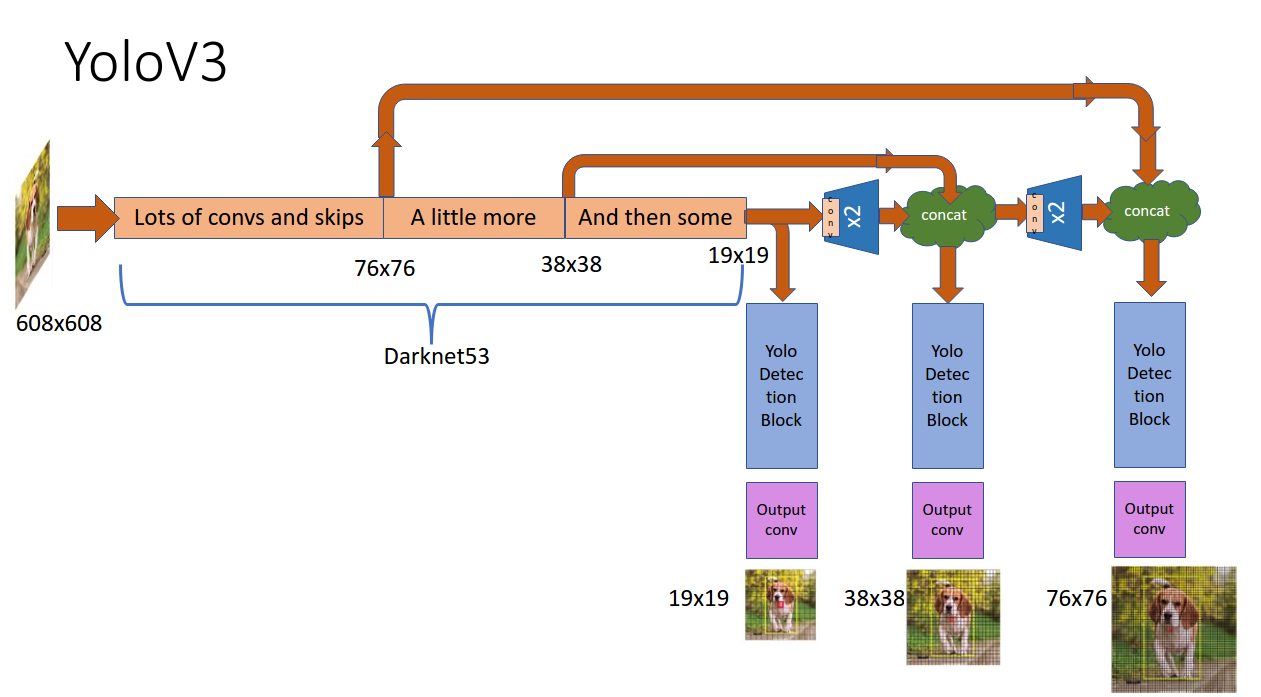
\includegraphics[width=0.7\textwidth]{images/yolov3_architecture.png}
\end{column}

\begin{column}{0.6\textwidth}
{\small
\begin{columns}[T]
\begin{column}{0.5\textwidth}
\textbf{\textcolor{blue!70}{YOLOv1}} (2016)

Первая одностадийная, 7$\times$7 grid

\vspace{0.2em}
\textbf{\textcolor{green!50!black}{YOLOv2}} (2017)

Anchor boxes, Darknet-19, 80 классов

\vspace{0.2em}
\textbf{\textcolor{blue!70}{YOLO9000}} (2017)

WordTree $\to$ 9000 классов

\vspace{0.2em}
\textbf{\textcolor{green!50!black}{YOLOv3}} (2018)

Darknet-53, 3 масштаба

\vspace{0.2em}
\textbf{\textcolor{blue!70}{YOLOv4}} (2020)

CSPDarknet53
\end{column}

\begin{column}{0.5\textwidth}
\textbf{\textcolor{green!50!black}{YOLOv5}} (2020)

PyTorch, 5 размеров

\vspace{0.2em}
\textbf{\textcolor{blue!70}{YOLOv8}} (2023)

Anchor-free, Mosaic v3

\vspace{0.2em}
\textbf{\textcolor{green!50!black}{YOLO-NAS}} (2023)

Neural Architecture Search
\end{column}
\end{columns}
}
\end{column}
\end{columns}
\end{frame}

% Слайд 10: SSD
\begin{frame}{SSD: Single Shot MultiBox Detector}
\begin{columns}[T]
\begin{column}{0.45\textwidth}
{\bfseries\textcolor{blue!70}{Multi-scale Detection}}

{\small Несколько feature maps разного разрешения}

{\small
\begin{itemize}
    \item Низкое разрешение $\to$ крупные объекты
    \item Высокое разрешение $\to$ мелкие объекты
\end{itemize}
}

\vspace{0.3em}
{\bfseries\textcolor{green!50!black}{SSD vs YOLO}}

{\small SSD: лучше на разных масштабах}

{\small YOLO: быстрее}
\end{column}

\begin{column}{0.55\textwidth}
{\bfseries\textcolor{blue!70}{Default Boxes (Anchors)}}

{\small Разные aspect ratios [1, 2, 3, 1/2, 1/3]}

{\small Предсказания: Offsets + Confidence}

\vspace{0.3em}
{\bfseries\textcolor{green!50!black}{Архитектура}}

{\small
\begin{itemize}
    \item Backbone: VGG16
    \item Extra layers для разных масштабов
    \item Prediction: классификация + локализация
\end{itemize}
}

\vspace{0.3em}
{\bfseries\textcolor{blue!70}{Loss:}} Confidence + Localization
\end{column}
\end{columns}
\end{frame}

% Слайд 11: FPN
\begin{frame}{FPN: Feature Pyramid Network}
\begin{columns}[T]
\begin{column}{0.4\textwidth}
{\bfseries\textcolor{blue!70}{Идея}}

{\small Объединение высокого разрешения с высокоуровневой семантикой}

\vspace{0.5em}
\centering
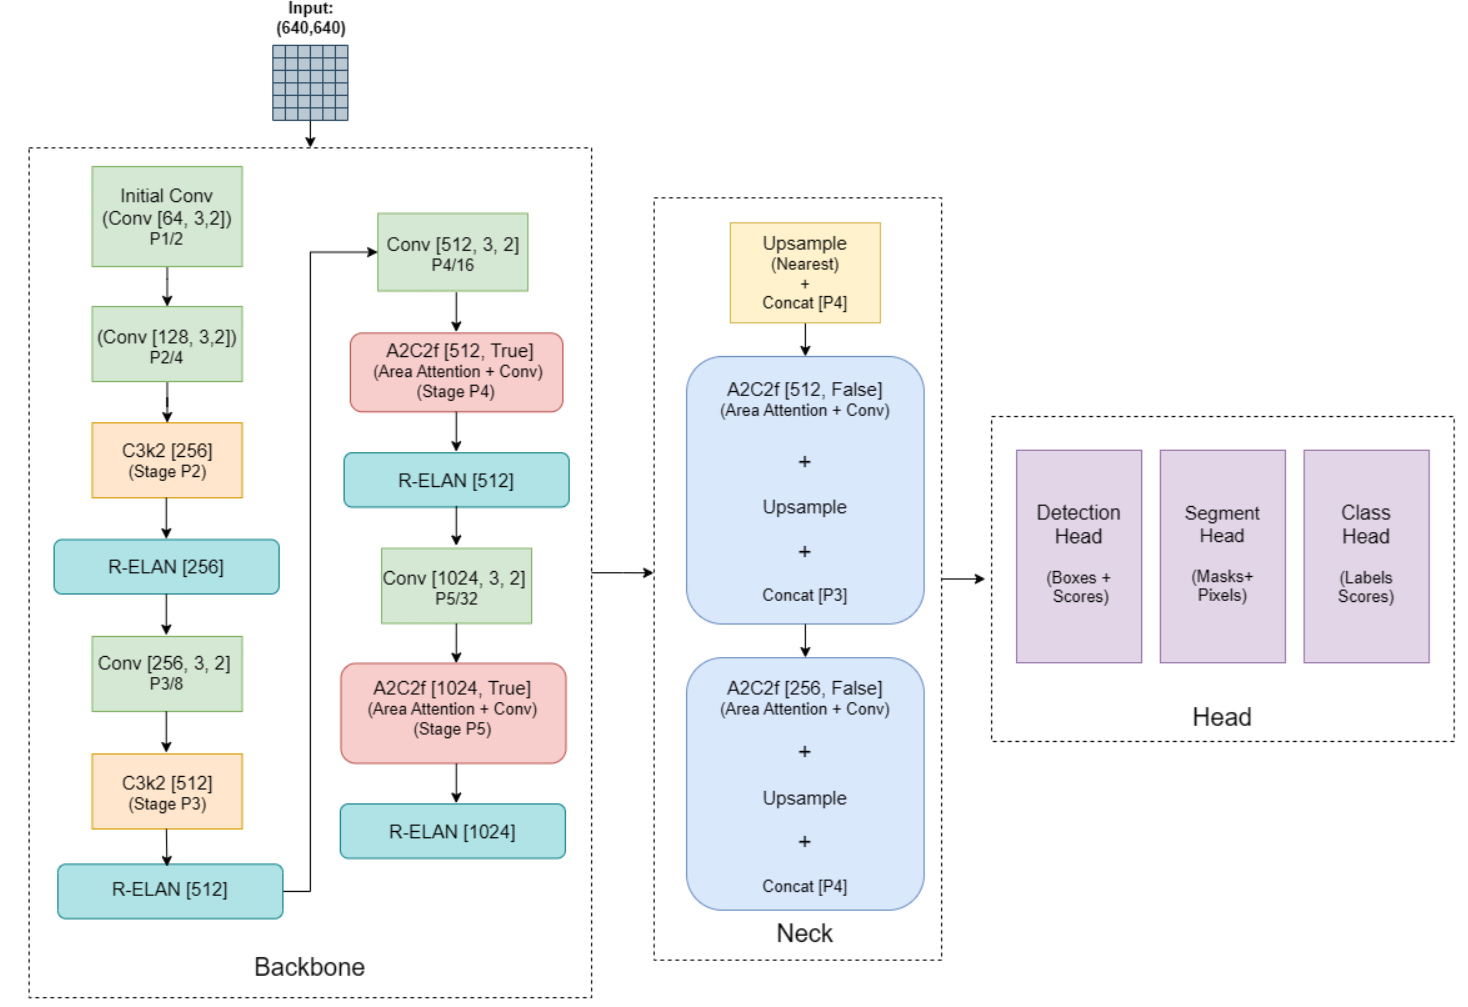
\includegraphics[width=0.7\textwidth]{images/fpn_architecture.png}
\end{column}

\begin{column}{0.6\textwidth}
{\bfseries\textcolor{blue!70}{Проблема}}

{\small Ранние слои: высокое разрешение, низкоуровневые признаки}

{\small Поздние слои: низкое разрешение, семантика}

\vspace{0.3em}
{\bfseries\textcolor{green!50!black}{Решение}}

{\small
\begin{itemize}
    \item Bottom-up: Forward pass $\to$ C2, C3, C4, C5
    \item Top-down: Upsample + lateral $\to$ P2, P3, P4, P5
\end{itemize}
}

\vspace{0.3em}
{\bfseries\textcolor{blue!70}{Преимущества}}

{\small Детекция объектов разных размеров}

{\small Используется в: Faster R-CNN + FPN, Mask R-CNN}
\end{column}
\end{columns}
\end{frame}

% Слайд 12: Сегментация
\begin{frame}{Архитектуры для сегментации}
\begin{columns}[T]
\begin{column}{0.45\textwidth}
{\bfseries\textcolor{blue!70}{U-Net}}

{\small
\begin{itemize}
    \item \textbf{Encoder:} сжимает изображение
    \item \textbf{Bottleneck:} сжатая семантика
    \item \textbf{Decoder:} восстанавливает
\end{itemize}
}

{\small Skip connections: encoder $\to$ decoder}

\vspace{0.3em}
{\bfseries\textcolor{green!50!black}{Почему работает?}}

{\small Encoder: изучает «что»}

{\small Decoder: изучает «где»}
\end{column}

\begin{column}{0.55\textwidth}
{\bfseries\textcolor{blue!70}{Mask R-CNN}}

{\small Faster R-CNN + ветка для масок}

{\small
\begin{itemize}
    \item ROI Align: точное выравнивание
    \item Три выхода: класс + bbox + маска
\end{itemize}
}

\vspace{0.5em}
\centering
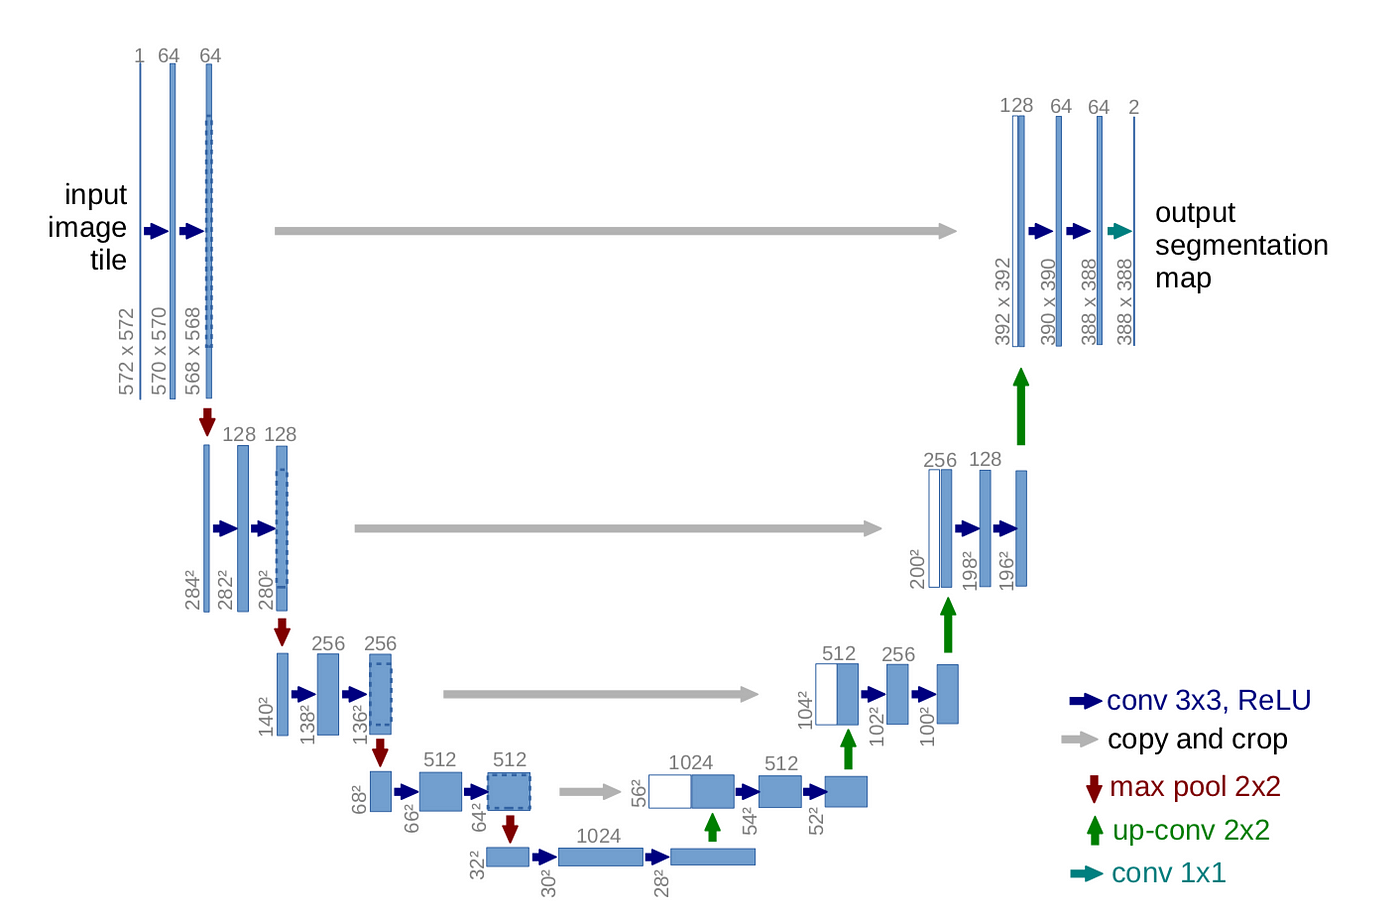
\includegraphics[width=0.6\textwidth]{images/unet_architecture.png}
\end{column}
\end{columns}
\end{frame}

% Слайд 13: DeepLab
\begin{frame}{DeepLab: семантическая сегментация}
\begin{columns}[T]
\begin{column}{0.45\textwidth}
{\bfseries\textcolor{blue!70}{Atrous Convolution}}

{\small Увеличивает receptive field без роста параметров}

{\small rate=2: каждый 2й пиксель}

{\small rate=4: каждый 4й пиксель}

\vspace{0.3em}
{\bfseries\textcolor{green!50!black}{ASPP}}

{\small Параллельные свертки с rates 1, 6, 12, 18}

{\small Захват объектов разных масштабов}
\end{column}

\begin{column}{0.55\textwidth}
{\bfseries\textcolor{blue!70}{Encoder-Decoder}}

{\small
\begin{itemize}
    \item Encoder: Backbone + ASPP
    \item Decoder: Upsample + признаки
    \item Bilinear upsample 4x
\end{itemize}
}

\vspace{0.3em}
{\bfseries\textcolor{green!50!black}{Deep Supervision}}

{\small Auxiliary loss на промежуточных слоях}

\vspace{0.3em}
{\bfseries\textcolor{blue!70}{Применение}}

{\small Медицина, спутники, автономное вождение}
\end{column}
\end{columns}
\end{frame}

% Слайд 14: Генеративные модели
\begin{frame}{Генеративные модели}
\begin{columns}[T]
\begin{column}{0.55\textwidth}
{\bfseries\textcolor{blue!70}{GAN}}

{\small Generator создает, Discriminator оценивает}

{\small Адверсарное обучение}

\vspace{0.3em}
{\bfseries\textcolor{green!50!black}{Diffusion Models}}

{\small Forward: добавляет шум}

{\small Reverse: удаляет шум пошагово}

{\small U-Net предсказывает шум}

\vspace{0.3em}
{\bfseries\textcolor{blue!70}{VAE}}

{\small Encoder $\to$ Latent Space $\to$ Decoder}
\end{column}

\begin{column}{0.45\textwidth}
{\bfseries\textcolor{blue!70}{Применение}}

{\small
\begin{itemize}
    \item GAN: StyleGAN, pix2pix
    \item Diffusion: DALL-E, Stable Diffusion
    \item Text-to-image генерация
    \item Inpainting, Super-resolution
\end{itemize}
}

\vspace{0.3em}
{\bfseries\textcolor{green!50!black}{Отличия}}

{\small GAN: адверсарная игра}

{\small Diffusion: пошаговое удаление шума}

{\small VAE: сжатие в latent space}
\end{column}
\end{columns}
\end{frame}

% Слайд 15: Применение
\begin{frame}{Применение Computer Vision}
\begin{columns}[T]
\begin{column}{0.5\textwidth}
{\bfseries\textcolor{blue!70}{Медицина}}

{\small Сегментация опухолей, классификация рентгена}

\vspace{0.3em}
{\bfseries\textcolor{green!50!black}{Автономное вождение}}

{\small Детекция объектов, сегментация дороги}

\vspace{0.3em}
{\bfseries\textcolor{blue!70}{Промышленность}}

{\small Контроль качества, сортировка продукции}

\vspace{0.3em}
{\bfseries\textcolor{green!50!black}{Сельское хозяйство}}

{\small Мониторинг посевов, детекция болезней}
\end{column}

\begin{column}{0.5\textwidth}
{\bfseries\textcolor{blue!70}{Безопасность}}

{\small Face recognition, детекция аномалий}

\vspace{0.3em}
{\bfseries\textcolor{green!50!black}{Медицинская визуализация}}

{\small Сегментация органов, анализ КТ/МРТ}

\vspace{0.5em}
\centering
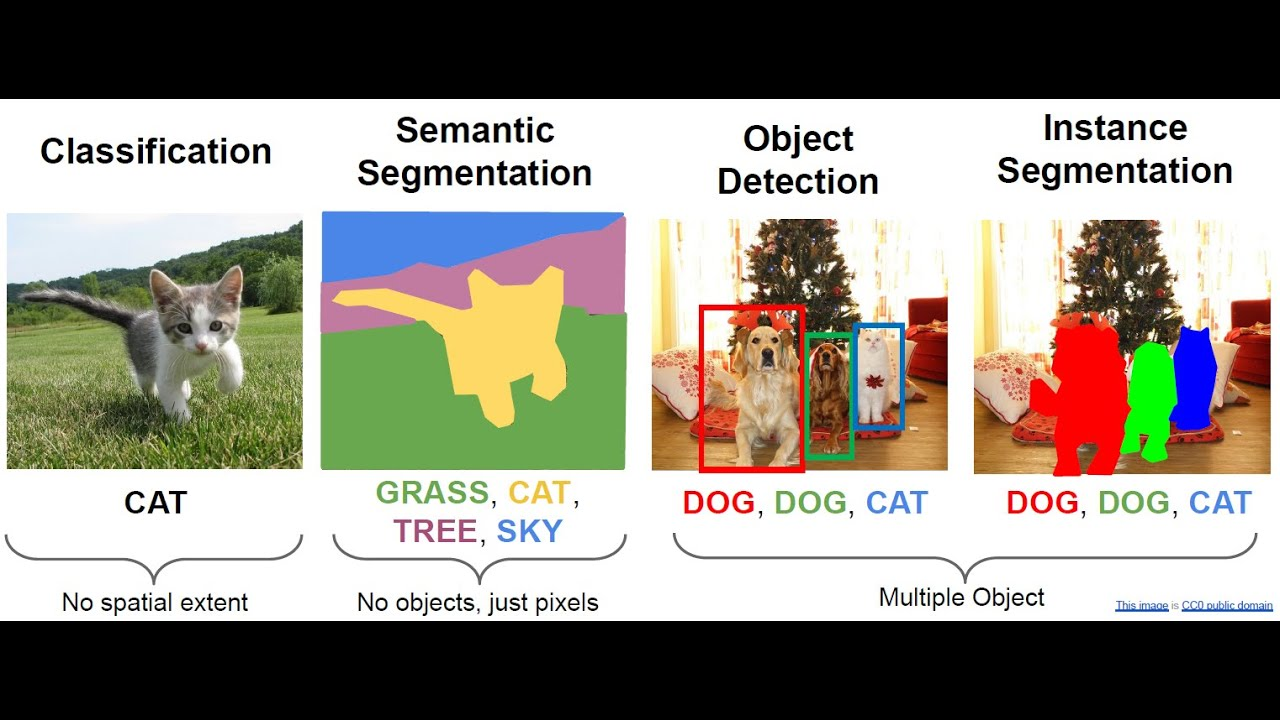
\includegraphics[width=0.6\textwidth]{images/cv_applications.png}
\end{column}
\end{columns}
\end{frame}

% Слайд 16: Заключение
\begin{frame}{Перспективы развития}
\begin{columns}[T]
\begin{column}{0.4\textwidth}
{\bfseries\textcolor{blue!70}{Выводы}}

{\small
\begin{itemize}
    \item Нейросети — стандарт в CV
    \item Выбор архитектуры под задачу
    \item Понимать принципы работы
\end{itemize}
}

\vspace{0.5em}
\centering
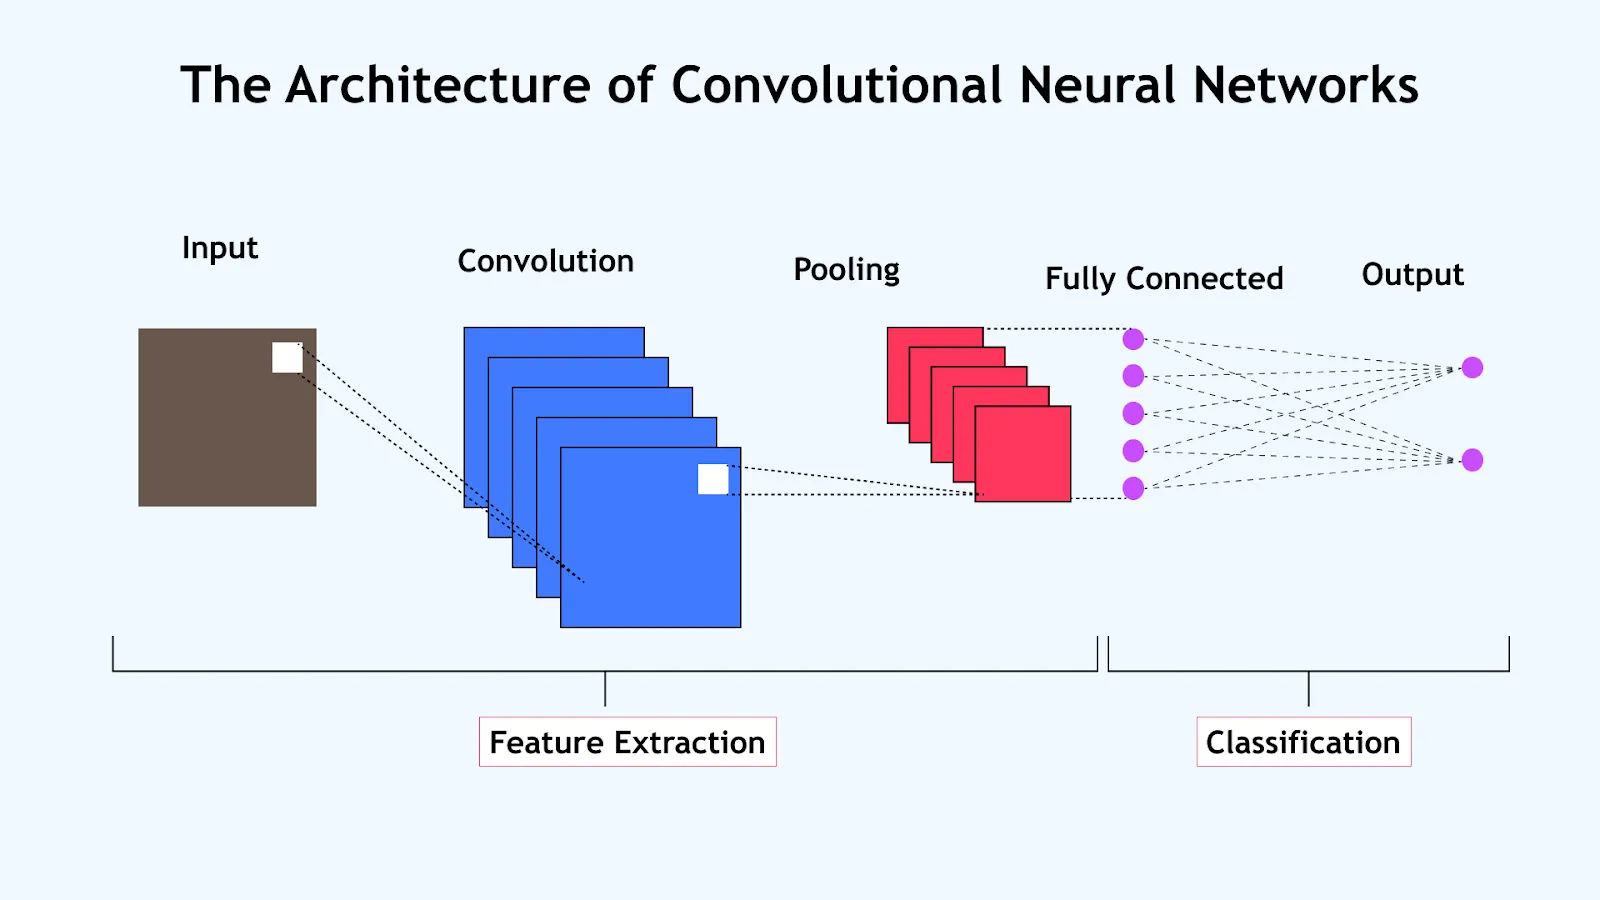
\includegraphics[width=0.7\textwidth]{images/cnn_architecture.png}
\end{column}

\begin{column}{0.6\textwidth}
{\bfseries\textcolor{blue!70}{Современные тренды}}

{\small
\begin{itemize}
    \item Transfer Learning: предобученные модели
    \item Vision Transformers: patches + attention
    \item Мультимодальность: CLIP, DALL-E
    \item Self-supervised: обучение без разметки
    \item Explainable AI: Grad-CAM
    \item Генеративные модели: GAN, Diffusion
\end{itemize}
}

\vspace{0.3em}
{\small\textbf{Главное:} Понимать принципы работы архитектур, а не просто применять готовые модели}
\end{column}
\end{columns}
\end{frame}

\end{document}